\documentclass[8pt]{beamer}
\usetheme{default} % Very simple theme
\usecolortheme{dove} % Minimalist grayscale colors
\setbeamertemplate{navigation symbols}{} % Remove navigation bar

% Define brand-like colors
\definecolor{myblue}{RGB}{0, 102, 204}    % Blue for standard blocks
\definecolor{mygreen}{RGB}{0, 153, 0}     % Green for example blocks
\definecolor{myred}{RGB}{204, 0, 0}       % Red for alert blocks
\definecolor{myorange}{RGB}{255, 128, 0} % For \emph

% Accent color for titles, bullets, etc.
\setbeamercolor{structure}{fg=myblue}

% Block colors
\setbeamercolor{block title}{bg=myblue, fg=white}
\setbeamercolor{block body}{bg=blue!5, fg=black}

\setbeamercolor{exampleblock title}{bg=mygreen, fg=white}
\setbeamercolor{exampleblock body}{bg=green!5, fg=black}

\setbeamercolor{alertblock title}{bg=myred, fg=white}
\setbeamercolor{alertblock body}{bg=red!5, fg=black}
\setbeamercolor{alerted text}{fg=myred}

% Optional: color for \example text
\setbeamercolor{example text}{fg=mygreen}

% Custom emph (orange text instead of italic)
\let\oldemph\emph
\renewcommand{\emph}[1]{\textcolor{myorange}{#1}}
\newcommand{\ve}[1]{\boldsymbol{#1}}

\usepackage{graphicx} % Package for images
\usepackage{amsmath} % Package for images
\graphicspath{{figs/}} % Path to your figures directory
\usepackage{array}  % For better column spacing
\usepackage{caption} % Required for \captionof

% Title Information
\title{STOCHASTIC METHODS IN WATER RESOURCES}
\vspace{25pt}
\subtitle{Unit 4: Time series analysis \\ Lecture 15: Special properties and models}
\author{Luis Alejandro Morales, Ph.D.}
\institute{Universidad Nacional de Colombia \\ Department of Civil and Agriculture Engineering} %// }
%\date{\today}

\begin{document}

% Title Slide
\begin{frame}
    \titlepage
\end{frame}

%-------
% From Kotte (Stochastic WR tech)
\section{Runs and crossing properties}
\begin{frame}{Runs and crossing properties}
    \begin{block}{Generalities}
    \end{block}
    \begin{itemize}
        \item There does not appear to be universally accepted method of defining \alert{droughts} in hydrometeorology. However, one criterion which has practical significance pertains to the \emph{deficits} with respect to (or excursions below) a specified level or rate of flow in a river. 
        \item The duration of a deficit  is known  as a \alert{run length}. In general, a \alert{run} is defined as a sequence of observations of the same kind preceded and succeeded by one or more observations  of a different kind.
        \item Corresponding to the \emph{run length}, the magnitude of the deficit is known as a \emph{run sum}. Such characteristics of a \emph{time series} belong to a general class called \emph{crossing properties}. 
        \item To explain these specifically, consider the \emph{crossing level} $u$ in the figure bellow which shows a section $(0,T)$ of a \emph{stationary discrete time series} $\xi_t$ with zero mean and variance $\sigma_{\xi}^2$. 

    \end{itemize}
\end{frame}

\begin{frame}{Runs and crossing properties}
    \begin{block}{Generalities}
    \end{block}
 
            \begin{figure}[htbp]
                \centering
            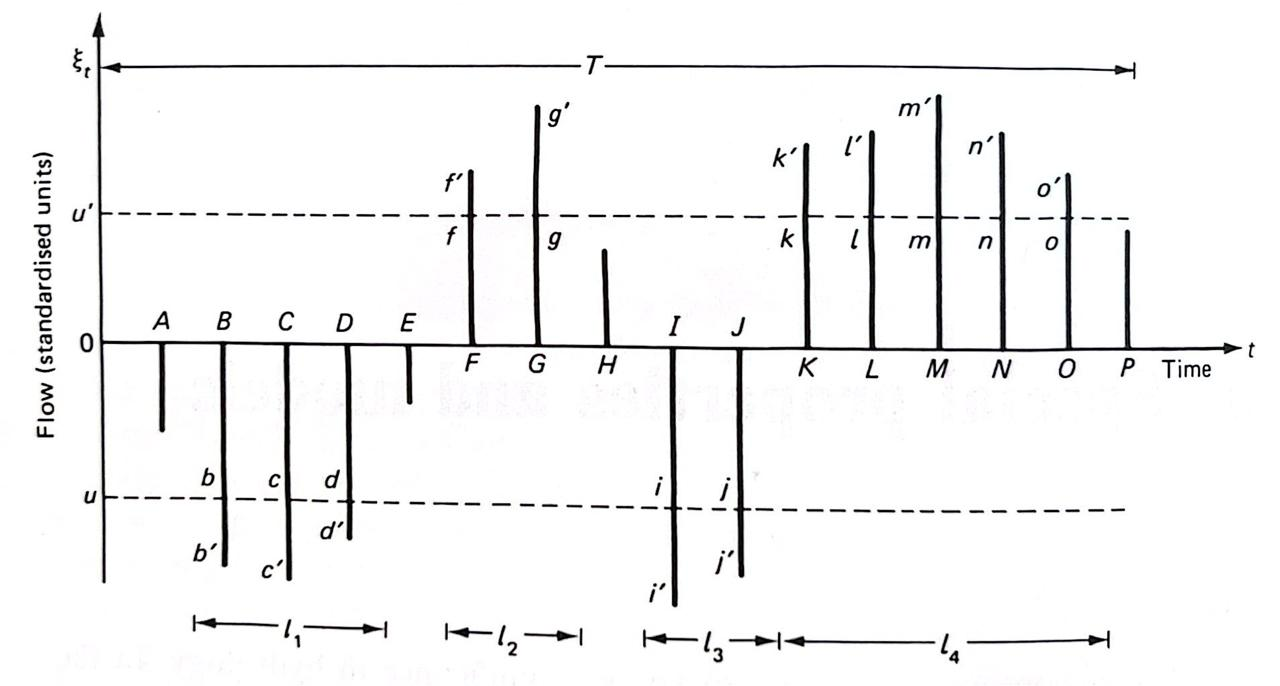
\includegraphics[width=\linewidth]{fiKo51.jpeg}  % from Kott
            \caption*{Crossing properties of a discrete time series, \emph{deficit run lengths} $l_1$, $l_3$ at level $u$; \emph{surplus run lengths} $l_2$, $l_4$ at level $u'$; downcrossings of level $u$ at $B$ and $I$ with \emph{deficit run sums} $bb' + cc' + dd'$ and $ii' + jj'$ respectively; \emph{upcrossings} of level $u'$ at $F$ and $K$ with \emph{surplus run sums} $f'f + g'g$ and $k'k + l'l + m'm + n'n + o'o$ respectively.}
            \end{figure}

\end{frame}
    
\begin{frame}{Runs and crossing properties}
    \vspace{-2pt}
    \begin{block}{Generalities}
    \end{block}
    \vspace{-5pt}
    \begin{itemize}
        \item Downcrossings of this level occur a times $B$ and $I$ because the flows at these times are less than $u$, whereas flows at the antecedent times $A$ and $H$ respectively are greater than $u$. 
    \item The corresponding  deficit  \emph{run lengths} are $l_1$ and $l_3$. Also, the quantities $bb' + cc' + dd'$ and  $ii' + jj'$ are known as the \emph{deficit run sums}.
    \item Here, $u$ can represent the \emph{level  in a river } which should be maintained in order to meet \emph{water supply demands}. Alternatively, $u$ may be relevant to the minimum \emph{rate of flow} required for \emph{pollution control}.  Again it could be the lowest acceptable \emph{level for navigation purposes}. 
    \item Then the \emph{deficit run sums} represent the quantities that need to be released, for example, from a \emph{regulating reservoir}. Furthermore, the design and operation of hydroelectrici schemes and the \emph{sizing of pumps} are related to \emph{crossings} and \emph{run sums}.  
    \item Likewise, the durations and magnitudes of flows above a fixed high levels such as $u'$ in the figure above, known as the surplus \emph{run lengths} and the \emph{sums} with respect to this level, are of importance for flood control purposes. 
    \item In the case shown, upcrossings of level $u'$  occur at times $F$ and $K$, and the surplus \emph{run lengths} are $l_2$ and $l_4$. The \emph{run sums}, given  by $f'f + g'g$, $k'k + l'l + m'm + n'n + o'o$ and so on, can be regarded as the storage reservation that needs to be made in a reservoir for the abatement of floods downstream. 
    \item Number of \emph{level crossings} too have an important physical relevance. The analysis of rare floods and, in general, the theory  of \emph{extreme values} are relevant to the crossings of levels remote from the mean. 
    \item In addition, the \emph{mean number of crossings} which characterise a time series are of interest to river engineers. 
    \item In general, the number of crossings at various levels, as well as the \emph{mean run lengths and sums}, are useful criteria in the analysis of time series.
    \end{itemize}
\end{frame}

 \begin{frame}{Runs and crossing properties}
    \begin{block}{Theoretical aspects}
    \end{block}
The \emph{theory of crossings} says that the expectations of the number of \emph{downcrossing} of a level $u$ (which is equal to the expectation of the number  of upcrossings of the same level) of a \emph{stationary normal stochastic process} $\xi_t$ with zero mean and variance $\sigma_{\xi}^2$ in an interval $0 \leq t \leq T$ is given by
\begin{equation}
    E[N_{T}^- (u) ] = T(2\pi)^{-1} \left( \frac{\lambda_2}{\sigma_{\xi}^2} \right)^{1/2} e^{-\frac{u^2}{2\sigma_{\xi}^2}}
    \label{e51}
\end{equation}
in which $\lambda_2$ is the \emph{second moment} of the \emph{spectral density function} $f(\omega)$, where $\omega$ is the \emph{frequency} in cycles per unit time; in general,
\[
    \lambda_r = \int_0^\infty \omega^r f(\omega) d\omega
\]
Also, if $C''(0)$ is the \emph{second derivative} of the \emph{covariance function} at the origin 
\begin{equation}
    \lambda_2 = -C''(0)
    \label{e52}
\end{equation}
 
It follows  that, for the \emph{mean level} ($u=0$), $E[N_{T}^- (0)] = T(2\pi)^{-1} \left[ -C''(0)/\sigma_{\xi}^2 \right]^{1/2}$ in this way, the \emph{mean number of crossings} of the zero level characterises a particular time series.

The applicability of equations such as equation~\ref{e51} is unfortunately limited because of the fundamental \emph{non-normal} nature of \emph{hydrologic time series}. Another apparent disadvantage is that practical investigations are made in discrete  time.
\end{frame}

 \begin{frame}{Runs and crossing properties}
    \begin{block}{Theoretical aspects}
    \end{block}
    If we consider again the discrete case shown in the figure above, let $L^{-} (u)$ and $S^{-} (u)$ denote a deficit \emph{run length } and deficit \emph{run sum}, respectively, in the interval $(0,T)$, where $T$ is large. As before, $N^{-}_T (u)$ denotes the number of downcrossings in $(0, T)$; this is also the number of \emph{deficit runs} in the same interval. If $Pr[\xi_{t-1} > u, \xi_t < u]$ is the probability of a \emph{downcrossing} at time $t$. The expected number of \emph{downcrossings} (or \emph{upcrossings} in $(0,T)$) is
\begin{equation}
    E[N_T^- (u)] = Pr[\xi_{t-1} > u, \xi_t < u] T
    \label{e53}
\end{equation}

For a discrete time series we can give the expected values of the \emph{deficit run length} and the \emph{deficit run sum} as follows.
\begin{equation}
    E[L^- (u)] = \frac{Pr[\xi_t < u]}{Pr[\xi_{t-1} > u, \xi_t < u]}
    \label{e54}
\end{equation}
and 
\begin{equation}
    E[S^- (u)] = E[L^- (u)] E[u-\xi_t | \xi_t  < u]
    \label{e55}
\end{equation}

where $|$ means conditional  to the inequality on the right. 

One purpose this can serve  is for comparing \emph{crossing properties} in generated and historical data as a means of testing the \emph{validity of postulate models}; the usefulness of such a procedure derives from the versatility of crossing properties. 
\end{frame}

 \begin{frame}{Runs and crossing properties}
     \begin{block}{Some properties of independent discrete series}
    \end{block}
    Consider an independent and identically distributed discrete series $X_t$, $t=1,2,3, \cdots$, which represents, say, the \emph{total precipitation} at a particular site during the tth year. Let $F(x)$ denote the common distribution function of the $X_t$ series. Also, let $q = F(u) = Pr[X \leq u]$, where $u$ is a crossing level and $p = 1-q$. Then, if $+1$ and $-1$ signify that $X_t$ is greater than (or equal to) $u$ and less than $u$ respectively, the probability distribution of \emph{surplus run lengths} is given by
    \begin{equation}
    \begin{aligned}
        Pr[L^+ = l] &= Pr \left[X_{i+2} = X_{i+3} = \cdots = X_{i+l} = 1, X_{i+l+1} = -1 | X_i = -1, X_{i+1} = 1 \right] \\
                    &= \frac{p^l q^2}{pq} = p^{l-1} q
    \end{aligned}
    \label{e56}
    \end{equation}
    for $l=1,2,3, \cdots$ which is a \emph{geometric distribution}. Also, it can be shown that the expected value and variance of \emph{surplus run lenghts} is 
    \begin{equation}
        E[L^+] = \frac{1}{q} \quad \quad var(L^+) = \frac{p}{q^2}
    \label{e57}
    \end{equation}

    Note that for \emph{deficit run lenghts} $L^-$ the probabilities $p$ and $q$ should be interchanged in equations~\ref{e56} and ~\ref{e57}. A useful outcomes is that the \emph{mean run length} is equal to 2 if the median value, for which $p=q=0.5$, is taken as the \emph{crossing level}. 

 
\end{frame}
 
 \begin{frame}{Runs and crossing properties}
     \begin{block}{Some properties of independent discrete series}
    \end{block}
     An alternative way to estimate \emph{runs} is to condition them on the number of $X$ values which are represented by $+1$ or $-1$. The expected total number and variance of \emph{runs}  $N= N_i^+ + N_i^-$ are then given by 
    \begin{equation}
    \begin{aligned}
        E[N] &= 1 + \frac{2nm}{n+m}\\
        var(N) &= \frac{2nm(2nm-n-m)}{(n+m)^2 (n+m-1)}
    \end{aligned}
    \label{e58}
    \end{equation}
    where $n$ and $m$ represent the numbers of values above and below the chosen \emph{crossing level}, respectively.
    
    If \emph{long runs} are observed in a given sequence, which is the same as having only few runs, it indicates some type of grouping due to a \emph{serial correlation}, to a \emph{periodic movement} or perhaps to a \emph{trend}. In fact, a \emph{run test} can be formulated to test for independence on the basis of equation~\ref{e58}. The significance test is made on the assumption that $N$ is \emph{normally distributed}, the \emph{null hypothesis} being that the sequence is \emph{independent}. 
\end{frame}

%-------
% From Kotte (Stochastic WR tech)
\section{Range analysis}
\begin{frame}{Range analysis}
    \begin{block}{Hurst phenomenon}
    \end{block}
    According to Hurst (1951), there is an approximate relationship  between the \emph{rescaled range} and the \emph{sample size}. For an observed sequence $x_1, x_2, \cdots, x_N$ with $E[x]= \mu$, the range is defined by 
    \begin{equation}
        r_N = max\left[0, max(x_1 + x_2 + \cdots + x_i - i\mu) \right] - min\left[0, min(x_1 + x_2 + \cdots + x_i - i\mu) \right] 
    \label{e513}
    \end{equation}
    This is sometimes referred to as the \emph{crude range}.

    It is advantageous for practical purposes to calculate the difference between the \emph{maximum} $d_N^+$ and the \emph{minimun}  $d_N^-$ of the accumulated departures from the sample mean $\bar{x} = \frac{1}{N} \sum_{i=1}^N x_i$. This gives the adjusted range $r_N^*$. Thus
\begin{equation}
r_N^* =  max(x_1 + x_2 + \cdots + x_i - i\bar{x})-min(x_1 + x_2 + \cdots + x_i - i\bar{x}) = d_N^+ + |d_N^-| 
    \label{e514}
    \end{equation}
    Note that, for $i=N$, the terms within each set of parentheses in equaution~\ref{e514} sum to 0, but this does not necessarily apply to the corresponding terms in equation~\ref{e513}; hence, we have the addition of two zeros in the equation for $r_N$. 

%    To understand the \emph{range} more clearly, consider a hypothetical situation in which the \emph{observed flows} sequence is routed through a \emph{reservoir} of capacity $r_N^*$ with \emph{initial storage} $|d_N^-|$ and a constant \emph{withdrawal rate} $\bar{x}$ (incluging losses) per unit time. Under these conditions, the reservoir will be full on one or more occasions without overflowing, it will empty at least once and the withdrawal rate will be maintained throughout.

\end{frame}

 \begin{frame}{Range analysis}
    \begin{block}{Hurst phenomenon}
    \end{block}
In order to compare the results from different observed sequences, the \emph{range} is divided by the \emph{standard deviation} $S_N$ estimated by 
\[
    s_N = \frac{1}{\sqrt{N}} \left[ \sum_{i=1}^N (x_i - \bar{x})^2 \right]^{1/2}
\]
to give the adjusted rescaled range

\begin{equation}
    r_N^{**} = \frac{r_N^*}{s_N}
    \label{e515}
    \end{equation}

    This division by the \emph{standard deviation} is a unique feature of \emph{Hurst's work}. Of greater significance is the relation
\begin{equation}
    r_N^{**} = \left(\frac{N}{2} \right)^K
    \label{e516}
    \end{equation}
    where $K$ is deemed to be a constant for an observed sequence, which he established empirically. It was found that the exponent $K$ varies from 0.46 to 0.96 with a mean of 0.73 and a \emph{standard deviation} of 0.09 in the sequences which \emph{Hurst} examined. For the individual groups of data analysed such as \emph{river flows} we expect less variation. 

\end{frame}

  \begin{frame}{Range analysis}
    \begin{block}{Hurst phenomenon}
    \end{block}
    \emph{Hurst} also derived the theoretically \emph{expected value} of the \emph{adjusted range}. He used some \emph{coin-tossing experiments} to show that, for independent \emph{standard normal} variates, the asymptotic result
\begin{equation}
    E[R_N^*] = \sqrt{\frac{\pi}{2}} \sqrt{N} \approx 1.253 \sqrt{N}
    \label{e517}
    \end{equation}
    holds. 

    Similarly, \emph{Feller (1951)} gave an independent and rigorous  derivations of the same result, which is applicable to \emph{stationary independent  random variables} with finite variance regardless of the distribution. Note that the result is valid only if $N$ is large, say, greater than 1000. He also showed that the variance of $R_N^{**}$ is 
\begin{equation}
    var(R_N^{**}) = \left(\frac{\pi^2}{6} - \frac{\pi}{2} \right) N = 0.074N
    \label{e518}
    \end{equation}
    This holds approximately for $N\geq 50$.

    Analogous to equation~\ref{e516}, the more general form
\begin{equation}
    E[R_N^{**}] = cN^h
    \label{e519}
    \end{equation}
    has been adopted by \emph{Mandelbrot and Wallis (1968)} in which the exponent $h$ is the \emph{Hurst coefficient} and $c$ is another constant. It was postulated that a \emph{natural process} is characterized by a population value $h$; the small sample estimate of $h$ is denoted by $H$. The fact that values of $H \ne 0.5$ are found in \emph{observed natural sequences}  whereas, for a \emph{normal independent} or \emph{ARMA} type process, the asymptotic value of $h$ is 0.5 has become known as the \alert{Hurst phenomenon}. 
\end{frame}

  \begin{frame}{Range analysis}
      \begin{block}{Estimation of Hurst coefficient $h$}
    \end{block}
    \begin{itemize}
        \item Mandelbrot and Wallis (1969) proposed a graphical procedure for estimating $h$, through a so-called pox diagram. This involves computations which use equation~\ref{e515} of \emph{rescaled range} $r_{t,n}^{**}$ based on different subsequence sizes $n\leq N$, from the same record, in contrast with the use of the complete sample size $N$ as in the estimation of $K$ from equation~\ref{e516}; $t$ denotes the starting points of the subsequence which are also varied.
        \item Computed values are plotted on a double logarithm  graph of $r_{t,n}^{**}$ againts $n$. If $\bar{R}_n^{**}$ denotes the \emph{estimated mean} of the $r_{t,n}^{**}$ with $n$ fixed and $t$ variable, the estimated $H$ of $h$ is the \emph{slope} of straight line fitted by eye to the plot of $\bar{R}_n^{**}$ against $n$ for $n > n_0$; here $n_0 \approx 20$ is taken as the arbitrary upper limit of the so-called initial transient stage.  
        \item For these computations, values of $t$ and $n$ are chosen so that the information abstracted is maximised as far as possible whilst minimizing the amount of overlapping between sequences.
        \item In general, estimates of $h$ are biased because the slope $h$ depends on $n$. That is, $E[\bar{R}_n^{**}] \approx n^{h(n)}$, whereas we are attempting to estimate $\lim_{n\rightarrow \infty} [h(n)] = h$, in which $h(n)$ is the \emph{local exponent}.
    \end{itemize}
\end{frame}

  \begin{frame}{Range analysis}
    \vspace{-5pt}
      \begin{block}{Range and rescaled range in small samples}
    \end{block}
    \vspace{-5pt}
    The interpretation of the \emph{Hurst phenomenon} given above, which is the commonly accepted one, is undoubtedly important from theoretical considerations. However, for practical purposes knowledge of the small sample behaviour of the \emph{range statistics} is required. 
    \begin{enumerate}
        \item \emph{Independent identically  distributed standard normal variate} are considered. For this adjusted range, it has been proved that
    \vspace{-5pt}
\begin{equation}
    E[R_N^*] = \sqrt{\frac{N}{2\pi}} \sum_{i=1}^{N-1} \left[i(N-i)\right]^{-1/2}
    \label{e520}
    \end{equation}

\item It has been stablished that, for the \emph{rescaled adjusted range} 
    \vspace{-5pt}
\begin{equation}
    E[R_N^{**}] = \sqrt{\frac{1}{\pi}} \left[\frac{\Gamma((N-1)/2)}{\Gamma(N/2)} \right] \sum_{i=1}^{N-1} \left[(N-i)/i\right]^{1/2}
    \label{e521}
    \end{equation}

Again, for a sequence of inputs from a \emph{gamma population} with a two-parameter density function $f(x) = x^{\gamma-1} e^{-x/\lambda} / \lambda^{\gamma} \Gamma(\gamma)$ (where $\gamma$ and $\lambda$ are the shape and scale parameters respectively). Accordingly
\begin{equation}
    E[R_N^{*}] = 2\gamma^{-1/2} N^{-\gamma N} \Gamma(\gamma N) \sum_{i=1}^{N-1} \left[ \frac{i^{i\gamma - 1} (N-i)^{\gamma(N-i)}}{\Gamma(i\gamma) \Gamma(N\gamma - i\gamma)}\right] \quad  N=1,2,3, \cdots
    \label{e522}
    \end{equation}
\end{enumerate}
One important outcome of the theoretical work on the rescaled range as given by equation~\ref{e521} is that for finite sequences of \emph{independent  normal variates} the exponent $h$ is equation~\ref{e519} is significantly greater than 0.5. The asymptotic value, $h=0.5$, is reached only when $N$ is much larger than the sample sizes found in practices. 
%Likewise, \emph{Hurst's exponent} $K$ defined by equation~\ref{e516} undergoes transitory behaviour but at a slower rate. 
\end{frame}
 

\begin{frame}{Range analysis}
    \begin{block}{Explanation of Hurst phenomenon and experiments}
    \end{block}
    \begin{itemize}
        \item As seen before, observed sequences are not, in essence, normally distributed. However, computer experiments show that the \emph{adjusted rescaled range} $r_N^{**}$ is seemingly insensitive to changes in the marginal distributions.
        \item This is the contrast with the \emph{adjusted range} $r_N^*$ which becomes independent of the distribution only when $N$ is large, perhaps greater than 1000 in highly  skewed data. 
        \item The important characteristics of natural time series is \emph{persistence}. This is the property by which high flows tend to follow high flows and low flows tend to follow low flows. 
        \item A particular method of measuring persistence is through the \emph{serial correlagram}. The effect of (positive) serial correlation on the \emph{adjusted rescaled range} can be demonstrated by generating data sets using the \emph{AR(p)} and the \emph{ARMA(p,q)} models.
        \item In this way $K(N)$ and $h(N)$ are found to take on values greater than those for independent variates. These differences increase with increases in the \emph{serial correlation}. 
        \item However, they decrease for very large sample sizes; furthermore, it has been shown analytically that when $N$ becomes very large the \emph{Hurst coefficient} tends to the asymptotic value of 0.5 for \emph{ARMA} processes. 
    \end{itemize}
\end{frame}

\begin{frame}{Range analysis}
    \begin{block}{Explanation of Hurst phenomenon and experiments}
    \end{block}
    \begin{itemize}
        \item It follows from all of this that the preasymptotic  periods, over which the \emph{Hurst coefficient} is greater than 0.5 are much larger than those from independent variates.
        \item From the practical point of view, because sample sizes investigated by \emph{Hurst} were less than 2000, it seems reasonable to assume that \emph{serial correlation} can, at least, partly account for the observed \emph{Hurst phenomenon}.
        \item To conclude, it can be said that both \emph{serial correlation} and \emph{non-stationarity} can account for the \emph{Hurst} effect over finite time horizons. Indeed, many natural processes seem to have both these properties in varying degrees so that it is difficult to identify the effect of each. 
    \end{itemize}
\end{frame}
\end{document}
